\documentclass[border=4pt]{standalone}
\usepackage{fontspec}
\usepackage{amsmath}
\usepackage{unicode-math}
\setmainfont{Latin Modern Roman}
\setmathfont{Latin Modern Math}
\usepackage{pgfplots}
\usepackage{pgfplotstable}
\pgfplotsset{compat=1.18}
\usepackage{tkz-euclide}
\usetikzlibrary{arrows.meta,calc,angles,quotes,patterns,3d,backgrounds}
\definecolor{ink}{HTML}{123428}
\definecolor{asy}{HTML}{475569}
\definecolor{mint}{HTML}{86e0bd}
\tikzset{asym/.style={asy, line width=0.9pt, dash pattern=on 5pt off 3.5pt},
         guide/.style={gray!70, line width=0.6pt, densely dotted},
         dot/.style={circle, inner sep=0pt, minimum size=5pt, draw=white, line width=0.5pt},
         odot/.style={circle, inner sep=0pt, minimum size=5.5pt, fill=white, line width=1pt},
         lab/.style={font=\footnotesize, inner sep=1.5pt, text=ink}}
\begin{document}
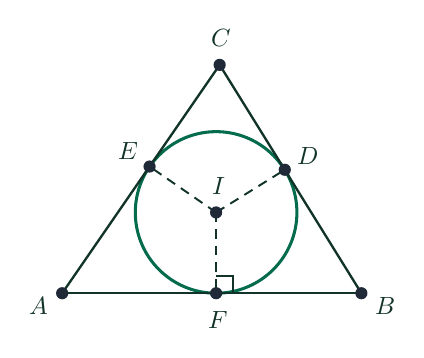
\begin{tikzpicture}
\draw[color={rgb,255:red,4;green,107;blue,77}, line width=1.1pt] (0.355,0.026) circle (1.026);
\draw[ink, line width=0.85pt] (-1.600,-1.000) -- (2.200,-1.000);
\draw[ink, line width=0.85pt] (2.200,-1.000) -- (0.400,1.900);
\draw[ink, line width=0.85pt] (0.400,1.900) -- (-1.600,-1.000);
\draw[ink, line width=0.7pt, dash pattern=on 3.5pt off 2.5pt] (0.355,0.026) -- (1.227,0.568);
\draw[ink, line width=0.7pt, dash pattern=on 3.5pt off 2.5pt] (0.355,0.026) -- (-0.490,0.609);
\draw[ink, line width=0.7pt, dash pattern=on 3.5pt off 2.5pt] (0.355,0.026) -- (0.355,-1.000);
\draw[ink, line width=0.7pt] (0.355,-0.780) -- (0.575,-0.780) -- (0.575,-1.000);
\fill[color={rgb,255:red,31;green,41;blue,55}] (-1.600,-1.000) circle (2.2pt);
\fill[color={rgb,255:red,31;green,41;blue,55}] (2.200,-1.000) circle (2.2pt);
\fill[color={rgb,255:red,31;green,41;blue,55}] (0.400,1.900) circle (2.2pt);
\fill[color={rgb,255:red,31;green,41;blue,55}] (0.355,0.026) circle (2.2pt);
\fill[color={rgb,255:red,31;green,41;blue,55}] (1.227,0.568) circle (2.2pt);
\fill[color={rgb,255:red,31;green,41;blue,55}] (-0.490,0.609) circle (2.2pt);
\fill[color={rgb,255:red,31;green,41;blue,55}] (0.355,-1.000) circle (2.2pt);
\node[font=\small, text=ink, inner sep=0.5pt] at (-1.902,-1.157) {$A$};
\node[font=\small, text=ink, inner sep=0.5pt] at (2.498,-1.163) {$B$};
\node[font=\small, text=ink, inner sep=0.5pt] at (0.409,2.240) {$C$};
\node[font=\small, text=ink, inner sep=0.5pt] at (0.381,0.365) {$I$};
\node[font=\small, text=ink, inner sep=0.5pt] at (1.515,0.749) {$D$};
\node[font=\small, text=ink, inner sep=0.5pt] at (-0.768,0.806) {$E$};
\node[font=\small, text=ink, inner sep=0.5pt] at (0.357,-1.340) {$F$};
\end{tikzpicture}
\end{document}
